\subsection{Block-Editor}
\begin{frame}
  \frametitle{\currentsectionname}

  \newtheorem{dev}{Entwicklungsziele}
  \begin{dev}
    \begin{itemize}
      \item Entwicklung eines Editors für Konvertierungen und SimplexSzenarios.
      \item Der Editor soll häufiges Nachschlagen verhindern.
      \item Der Editor soll Tippfehler vermeiden.
      \item Der Editor soll auch ohne SQL-Kenntnisse bedienbar sein.
    \end{itemize}
  \end{dev}

  % \note{
  %   \begin{itemize}
  %   \end{itemize}
  % }

\end{frame}

\begin{frame}
  \frametitle{\currentsectionname{} (cont.)}

  \begin{figure}
    \begin{center}
      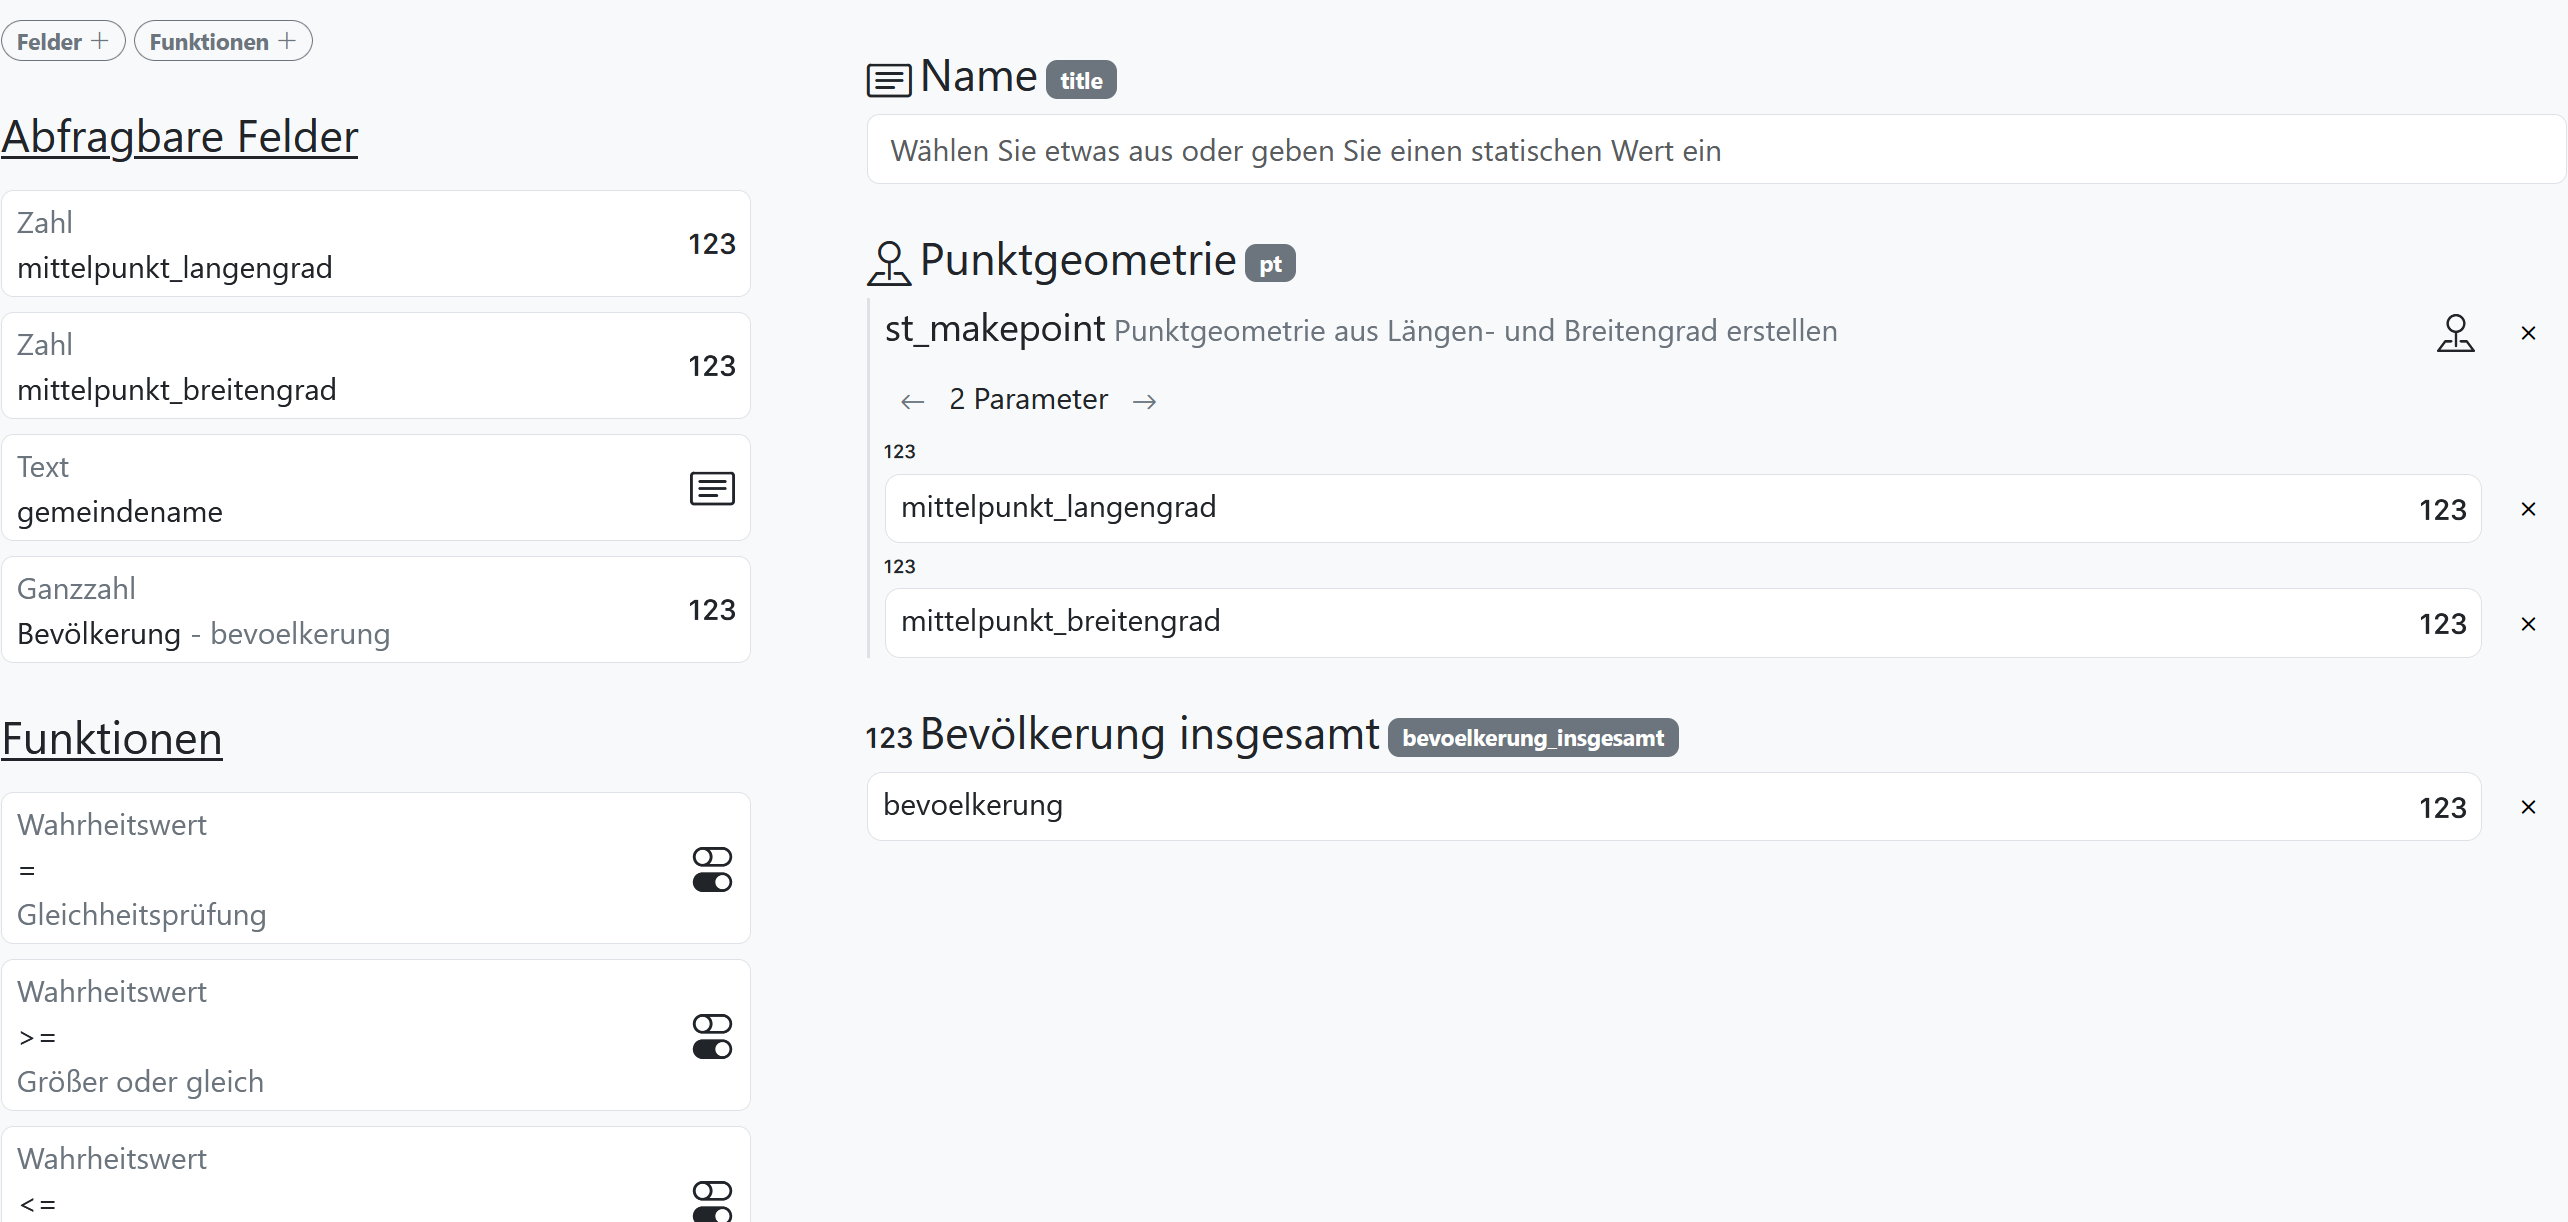
\includegraphics[width=0.95\textwidth]{assets/buffet-simple.png}
    \end{center}
    \caption{Bearbeitung einer Konvertierung im Block-Editor.}
  \end{figure}

\end{frame}
